\chapter{Theoretical background}
This chapter gives an overview over the most important distributions and transformations that are used for the SimpleSTORM algorithm and the Colorcomposer. An introduction to the most important parts of regular Charge-coupled Device (CCD) cameras is also given, as well as a section about the data the algorithm is designed for. 

\section{The data}
\subsection{Labeling}
The concept of direct stochastic optical reconstruction microscopy (dSTORM) (\cite{heilemann}) is, to label structures of interest with fluorophors that can be exited using a laser with the appropriate wavelength directly, in contrast to STORM techniques which need an additional activator fluorophore. Shortly after the activation the fluorophors emit a photon and fall back to the unexcited state or lose the ability to get exited, they bleach out. Special fluorophores have to be used that have a low probability to get activated. Each fluorophore is visible only every thousandth frame or even less frequently. A movie that shows the frames consecutively shows blinking spots.\newline
The technique to stain the samples that was used for all real-world images in this thesis is called immunofluorescence. For this technique antibodies are used to attach the fluorescenic molecules to the samples. Antibodies target specific biomolecules within a cell that show their antigen. There are two classes of immunofluorescence techniques.\newline
Primary immunofluorescence uses only one antibody that the fluorophore is directly attached to.\newline
For secondary immunofluorescence two kinds of antibodies are used. First the primary antibody that binds to the molecule or structure of interest and then a second antibody that binds to the primary and carries the fluorophore.

\subsection{Description of the data sets}
The datasets for dSTORM microscopy that we receive from our collaborators from
Bioquant, Heidelberg are big datasets of several gigabyte in the Andor ".sif" format. Each
file contains a stack of pictures, usually between 1000 and 10000, taken
consecutively with a fixed exposure time normally between 20 and 200 milliseconds. From now on the first two dimensions are called spatial dimensions. The third dimension of the data, resulting from the consecutive capturing of the images, is referred to as temporal dimension.\newline

Figure \ref{rawStorm} shows a typical frame of raw data. In each frame there might be multiple fluorophores visible at the same time. Due to the large magnification, beyond the diffraction limit, the almost pointlike fluorophores appear as approximately Gaussian shaped signals, their point spread functions. The fluorophores are either attached to the biological structures that are of interest or form a cluster, called a bead.\newline

Beads are larger and brighter than spots from only one fluorophore and are used to align multiple channels in the postprocessing step. Designed to show up in every frame of the sequence at the same position they can be used as landmarks for alignment. They are composed of fluorophores of different colors to be visible in every channel.\newline

The other spots, such as spots from fluorophores bound structures, often proteins of interest, only light up for a very short time. This is the key aspect of STORM. Instead of one frame that shows all fluorophores at the same time, thousands of frames are captured containing only a couple of point spread functions per frame. This makes it possible to determine the center of each point spread function with a sub-pixel precision. A high resolution image, with resolutions beyond the diffraction limit, can be reconstructed by plotting all detections found into one image.

\begin{figure}
\centering
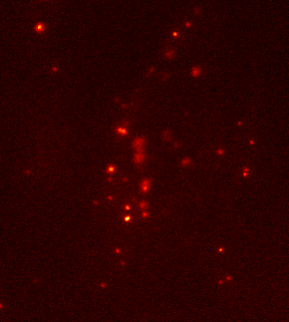
\includegraphics[width = 0.88\textwidth]{pictures/Pos2_2_red2-2frame2475Color.png}
	\caption{Raw image for dSTORM processing}
	\label{rawStorm}
\end{figure}


\section{Distributions}
\subsection{Gaussian distribution}
The one dimensional Gaussian distribution is characterized by its mean $\mu$ and its variance $\sigma^2$ which is its standard deviation squared. The probability density function is:
\begin{align}
f(x,\mu,\sigma) &= \frac{1}{\sqrt{2\pi}\sigma}\text{exp}\left(-\frac{(x-\mu)^2}{2\sigma^2}\right)&\text{1-D}
\end{align}
The $k$-dimensional probability density function is characterized by the covariance matrix$\Sigma$ and the is the $k$-dimensional mean $\pmb{\mu}$:
\begin{align}
f(x_1,...,x_k,\pmb{\mu},\Sigma)&=\frac{1}{\sqrt{(2\pi)^k \text{det}(\Sigma)}}\text{exp}\left(-\frac{1}{2}(\bf{x}-\pmb{\mu})^T\Sigma^{-1}(\bf{x}-\pmb{\mu})\right) &\text{$k$-D}
\end{align}
Figure \ref{poisgaussdistr} shows some Gaussian distributions. The two dimensional Gaussian distribution is used for the Gaussian filter.
\subsection{Poisson distribution}
A very important probability distribution in Physics is the Poisson
distribution. Its probability mass function is:
\begin{equation}
	p(n,\mu) = \frac{\mu^n}{n!}\exp(-\mu)
\end{equation}
The larger the mean value $\mu$ becomes the more likely the Poisson distribution results in a Gaussian distribution with a mean and a variance of $\mu$. Figure \ref{poisgaussdistr} shows Poisson and Gaussian distributions with different parameters. The mean value of the Gaussian was shifted by 0.5 which results from continuity correction.\newline
Poisson distributions describe the results of ``counting experiments'' and are
therefore important for image processing as pictures taken with a
camera are in principle counts of photons reaching the camera.  \newline
A Poisson distribution is defined for integer values only and its variance is
the same as the mean value of the distribution.\newline
The median of a Poisson distribution is approximately given by
\begin{align}
	\text{median Pois}(\lambda) \approx \lambda + \frac{1}{3} - \frac{1}{50\lambda} \label{meanMedianPoiss}
\end{align}
Another important attribute is
the skewness which describes the asymmetry of the distribution.
\begin{align}
 \text{skewness Pois}(\lambda) = \frac{1}{\sqrt{\lambda}}
\end{align}
The sum of Poisson-distributed independent variables is also Poisson-distributed.
\begin{figure}
\centering
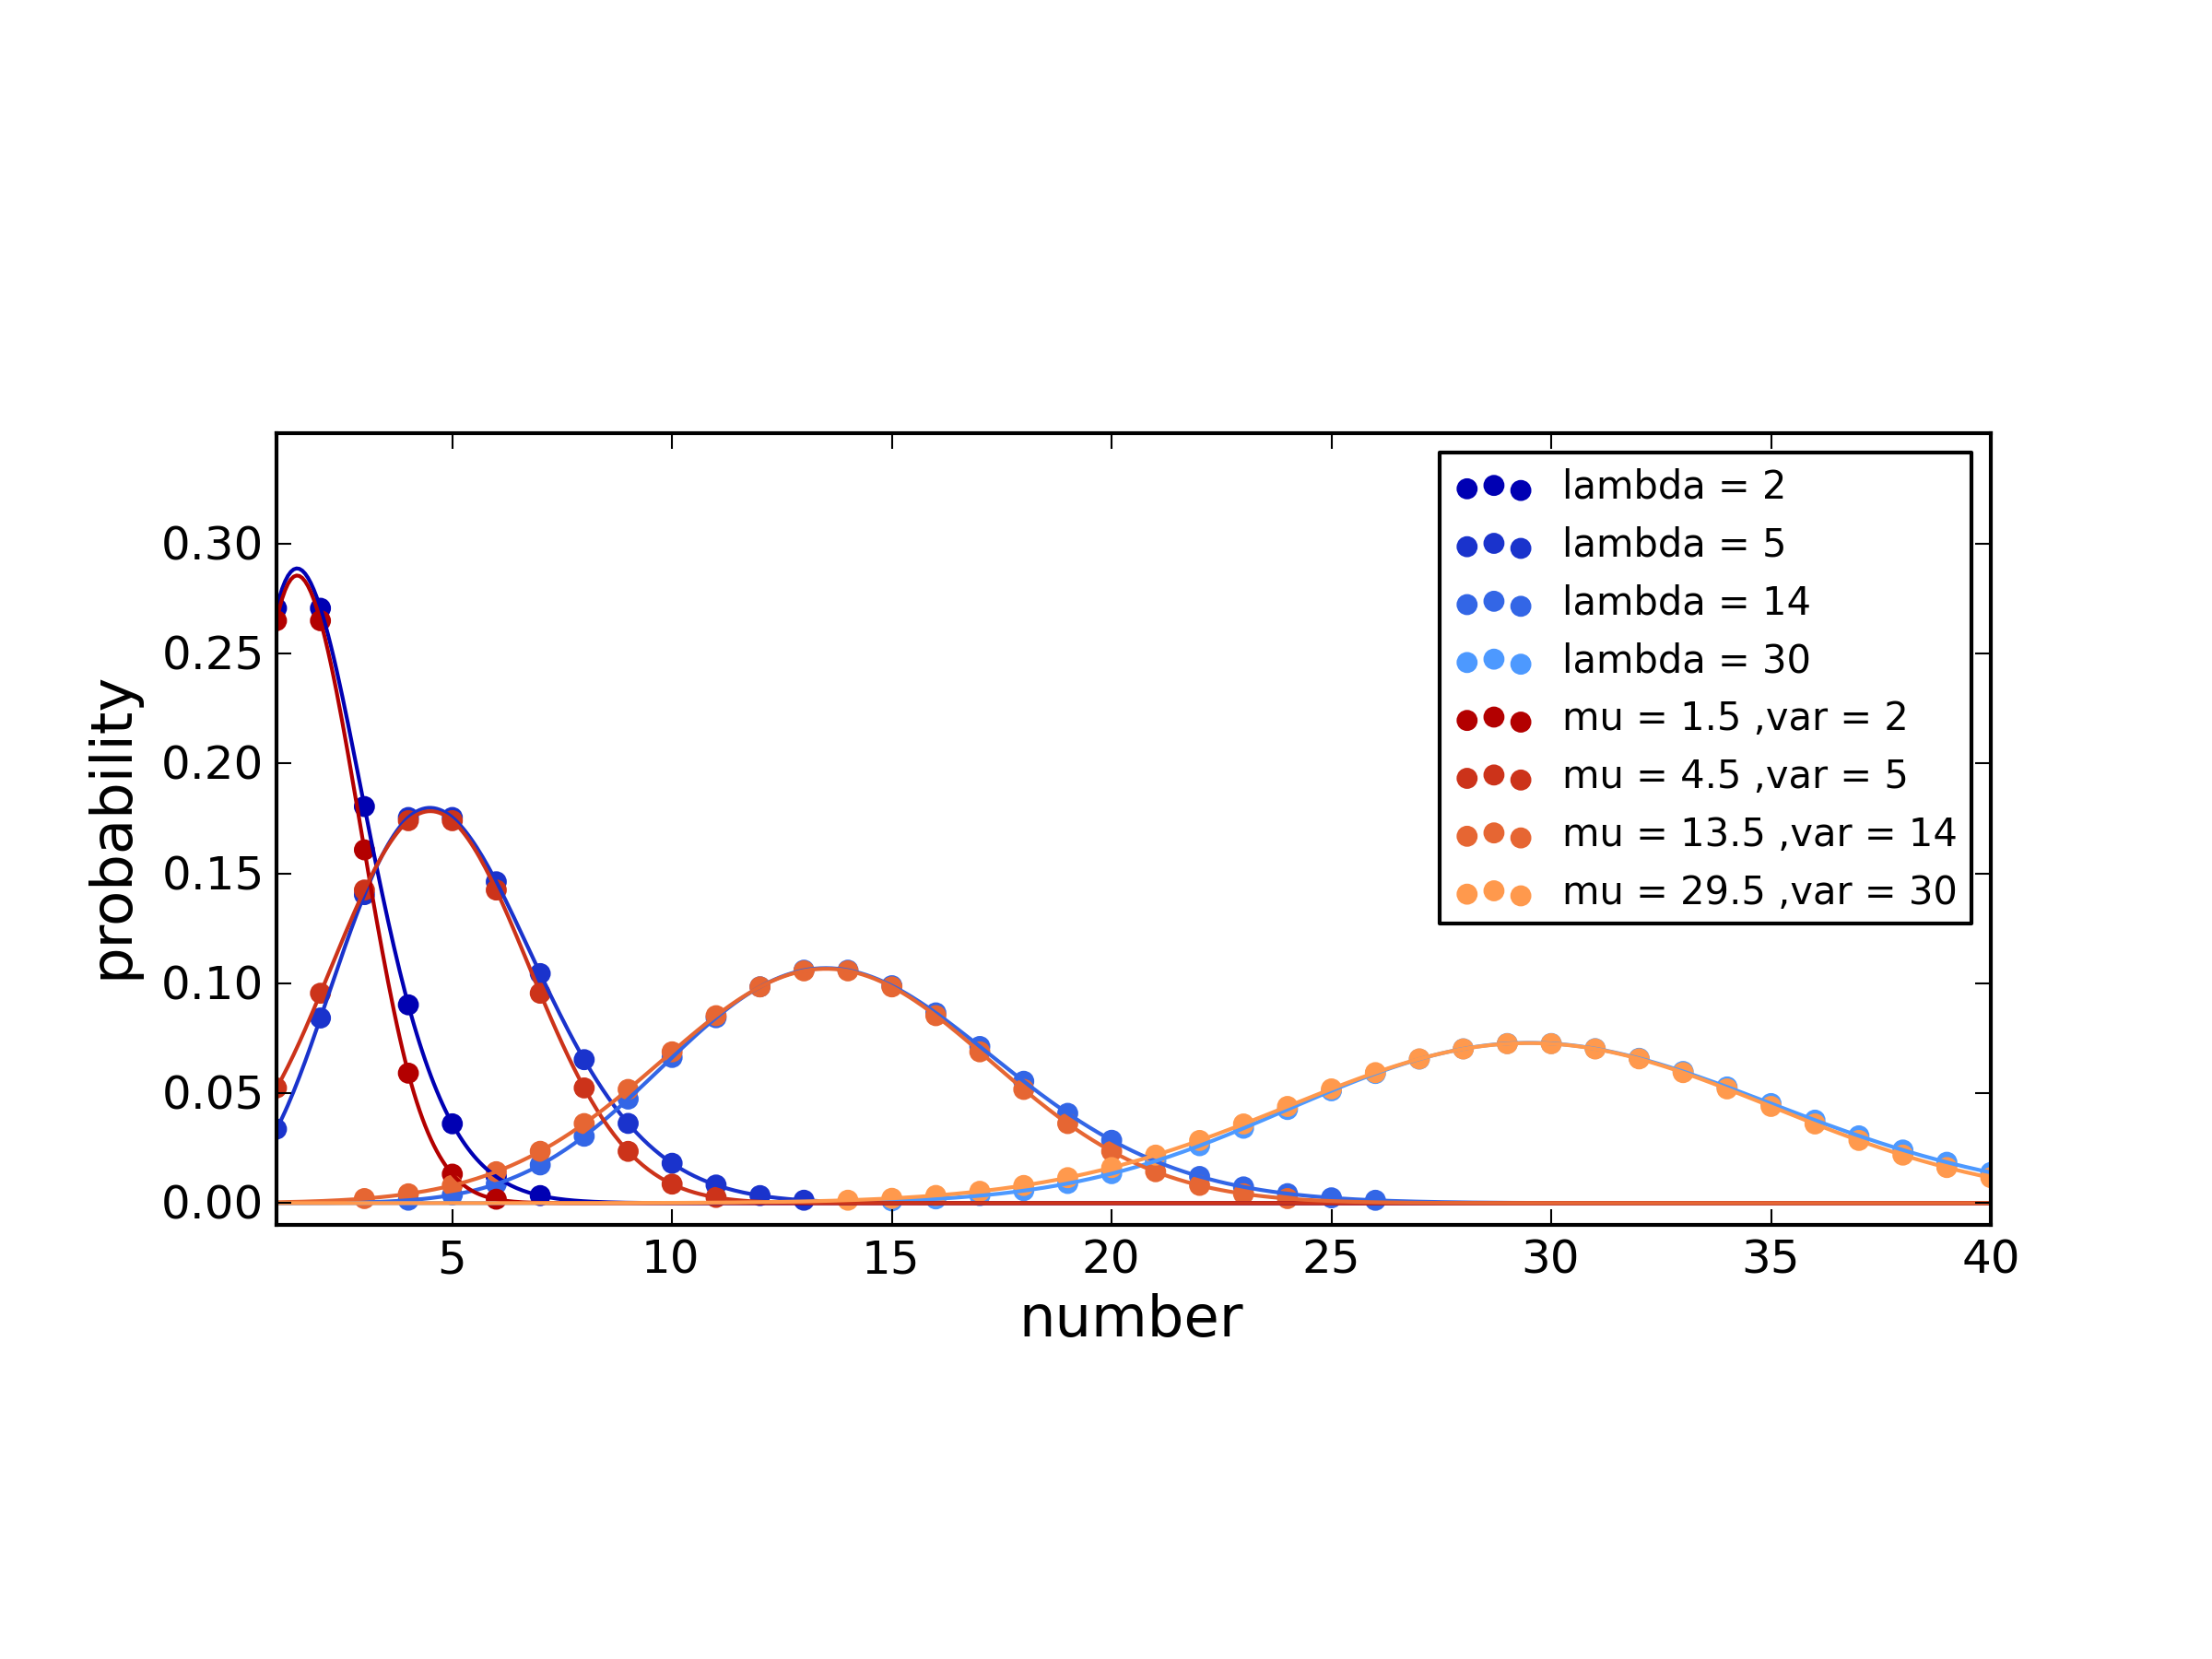
\includegraphics[width = 0.9\textwidth]{pictures/poissgaussdistr.png}
	\caption{Poisson and Gaussian distributions with different parameters. Especially for small numbers the Poisson and the Gaussian distribution differ. The larger $\mu$ gets for the Poisson distribution the more similar it gets to a Gaussian with mean $\mu$ and sigma $\sqrt{\mu}$. The Poisson distributions were interpolated between their defined values. For better comparison the integer values of the Gaussian distribution were also marked with dots.}
	\label{poisgaussdistr}
\end{figure}

\subsection{Skellam distribution}\label{skellamdist}
The variance of a Poisson distribution can be estimated using a Skellam distribution.
The probability
mass function of the Skellam distribution is a function of the difference between
two Poisson random variables
\begin{equation}
	p(k;\mu_1, \mu_2) =
	\exp(-(\mu_1+\mu_2))\left(\frac{\mu_1}{\mu_2}\right)^{k/2}~I_{|k|}\left(2\sqrt{\mu_1
	\mu_2}\right)
\end{equation}  
$\mu_1$ and $\mu_2$ are the means of two Poisson distributed random variables $n_1$ and $n_2$, $k = n_1 - n_2$.
$I_{|k|}$ is the modified Bessel function of the first kind.\\
Mean $\mu$ and variance $\sigma^2$ of the Skellam distribution are given by
\begin{align}
	&&\mu &= \mu_1 - \mu_2,& \sigma^2 &= \mu_1 + \mu_2\\
	\Rightarrow &&\mu_1& = \frac{\mu + \sigma^2}{2},& \mu_2 &=\frac{-\mu +
	\sigma^2}{2}
\end{align}
Figure \ref{skellamdistfig} shows two Poisson distributions ($P_\text{red}$ and $P_\text{blue}$) and the resulting Skellam distribution (purple) of the difference $P_\text{blue} - P_\text{red}$.
\begin{figure}
\centering
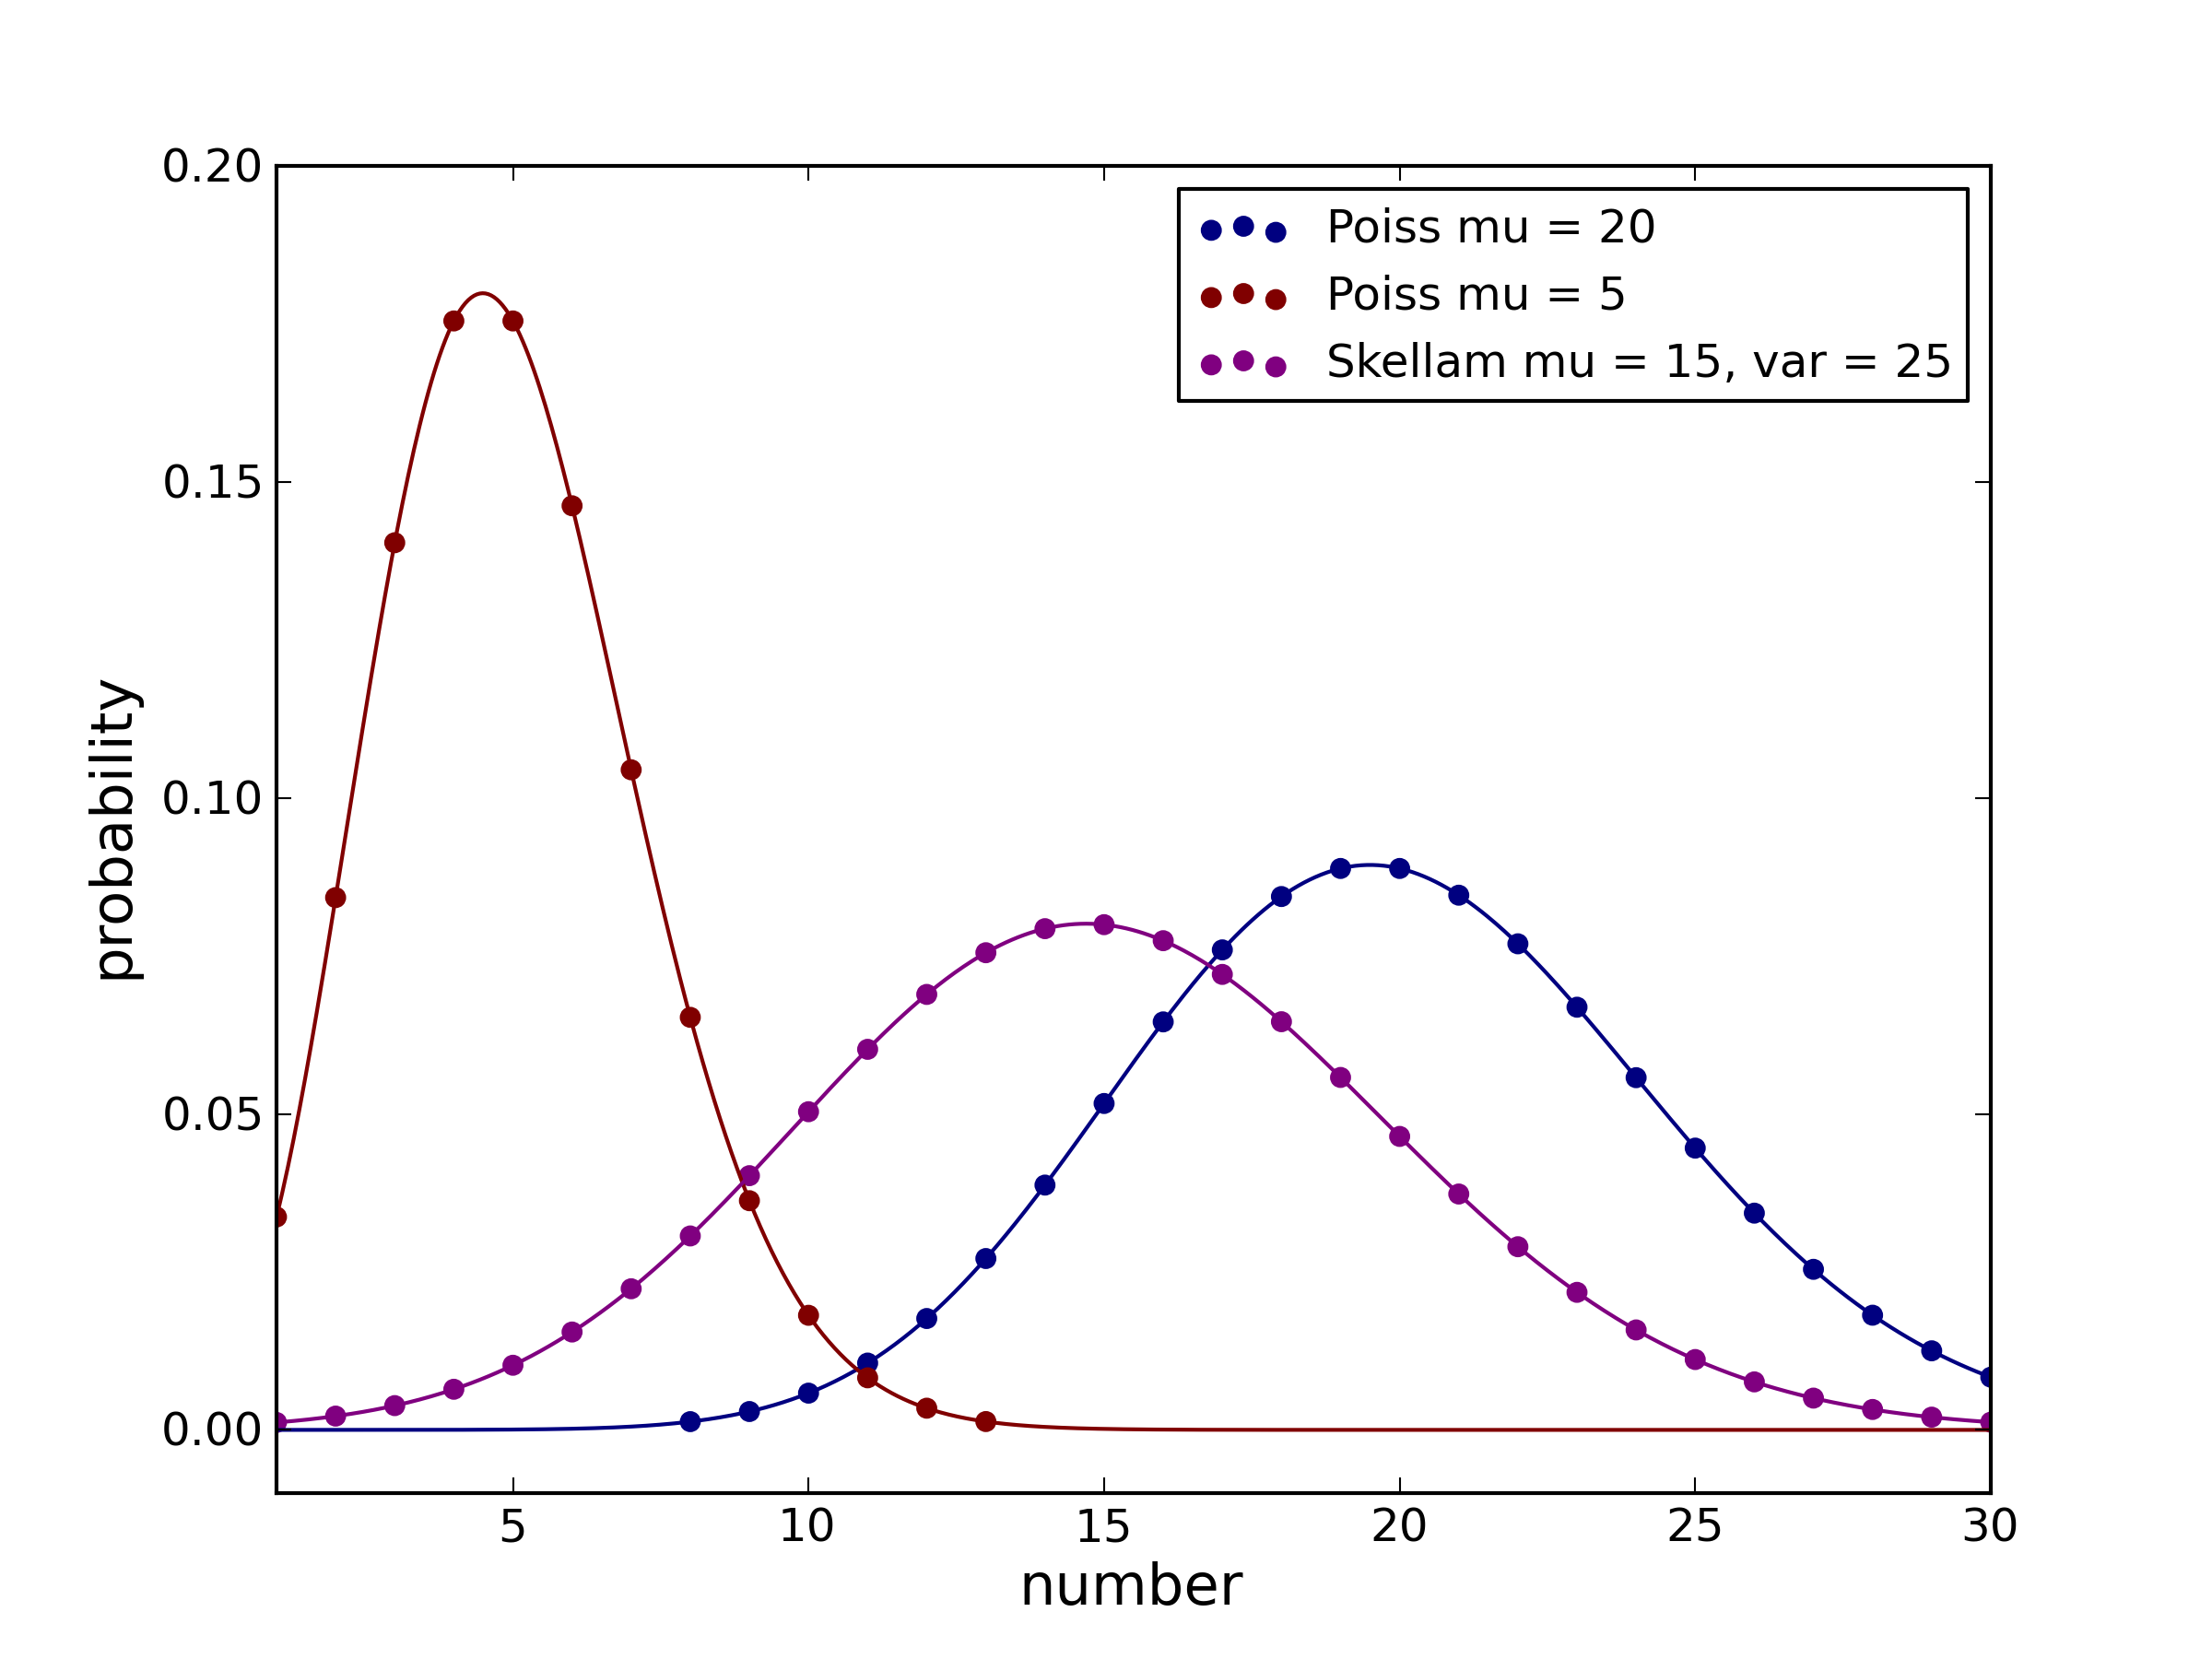
\includegraphics[width = 0.7\textwidth]{pictures/skellamdist.png}
	\caption{Two Poisson distributions and the resulting Skellam distribution. The distributions were interpolated between the integer values.}
	\label{skellamdistfig}
\end{figure}
If the differences between following values of a single Poisson distribution are used as $k$ for the Skellam distribution the variance of the Poisson distribution is given by the Skellam parameters $\mu_1$ or $\mu_2$ (the mean of the Skellam distribution $\mu$ will be close to zero if the same Poisson distributions are used).\newline
In section \ref{skellambettervariance} is shown which way to estimate the variance works better and more reliable.

\section{Charge-coupled Device (CCD) camera}
The light emitted by the fluorophores is captured by a CCD camera. During the capturing process the true measure, the photons arriving at the aperture of the camera, is transformed to electrons and eventually to a digital number. This section gives a short overview over the most important parts of the signal processing within a CCD camera.
\subsection{Photon counting noise}
The emission of photons is a random process that occurs at unpredictable times. Therefore the number of photons passing through a plane is never constant but varies around some average value. This means, that one can never determine exactly how many photons will hit the sensor chip of a CCD camera for example. This phenomena is called photon counting noise. It plays a major role if the total number of photons is low, for example from dark sources or with short exposure times of the camera.
\subsection{Quantum efficiency}
Quantum efficiency describes the fraction of photons creating a detectable electron in a sensor chip. The quantum efficiency depends on the wavelength of the incoming photon. Photons with energies below the band gap can not produce a free electron that can be detected. The quantum efficiency has a maximum for a certain wavelength. This maximum of the quantum efficiency is basically caused by two effects. The higher the energy of the photon is the higher is the kinetic energy of the freed electron and therefore the diffusion length is greater, but the electron is absorbed further from the detector and is more likely to recombine with an electron hole.
\subsection{Gain}
There are two different gain factors involved in the capturing process of a camera. Firstly the electric signal for each pixel may be amplified. Secondly there is a gain factor that describes the proportionality between collected electrons and the digital number it is associated with.
\subsection{Readout noise}
The origin of readout noise is the amplifier. The amplification is never perfect, this means that the exact number of electrons at the end of the amplification varies around the expected linearly increased value. There might also be some random signals in the electronics adding to the "true" signal. The readout noise does not depend on the exposure time.
\subsection{Dark current noise}
The dark current noise is generated by the thermal movement of the atoms in the sensor chip. The movement of molecules and atoms depends on the temperature of the material, therefore the dark current noise strongly depends on the temperature of the chip and can be reduced by cooling. Dark current noise generates electrons in the bins of each pixel, even with closed shutter. It increases constantly with time and follows Poisson statistics.
\subsection{Quantization}
The signal must fit into the output color depth. It has to be rounded or truncated to fit in. This process introduces errors that can be seen as additional noise that is dependent on the intensity of the signal. High intensities are disturbed less relative to low intensities.


\section{Transformations}
\subsection{Transformation to Poisson distributed signal} \label{trafoPoiss}
The images acquired from the camera do not show the real intensities
$I_\text{true}$, which result from the photon emission of the probe, but
transformed ones $I_\text{meas}$.\newline
A linear transformation of the data is assumed with two parameters, the gain $g$ and the offset $o$.
Incoming photons create electrons via inner photoelectric effect. These electrons
are collected for each pixel and might be amplified to get the final result.
Assuming a linear relation between the number of incoming photons and the number
of electrons created and a linear amplifier results in a factor $g$. This factor
is multiplied with the number of photons captured during exposure time for each
pixel.\\
There might also be a constant offset for the pixel intensities that is not affected by the gain factor.
If the gain factor $g$ and the offset $o$ are known the true intensity, the
number of photons detected is:
\begin{equation}
	I_\text{true} = \dfrac{I_\text{meas}-o}{g}. \label{transtopoiss}
\end{equation}
After this transformation the intensities of the background are assumed to be Poisson distributed.
\subsection{Anscombe transformation}
\label{trafoAnscombe}
The Anscombe transform (\cite{anscombe}) is used to transform a random variable with a Poisson
distribution into one with an approximately constant standard deviation. The
transformation is defined as:
\begin{equation}
	A(x) = 2\sqrt{x+\frac{3}{8}}
\end{equation}
Figure \ref{anscombe} shows the standard deviation of Poisson distributions with increasing mean (green line) and the standard deviation of Poisson distributions that are transformed useing the Anscombe transformation (blue line). As can be seen in Figure \ref{anscombe} the Anscombe transformations result has
an intensity independent standard deviation of one for mean intensities greater than 4.
\begin{figure}
	\centering
	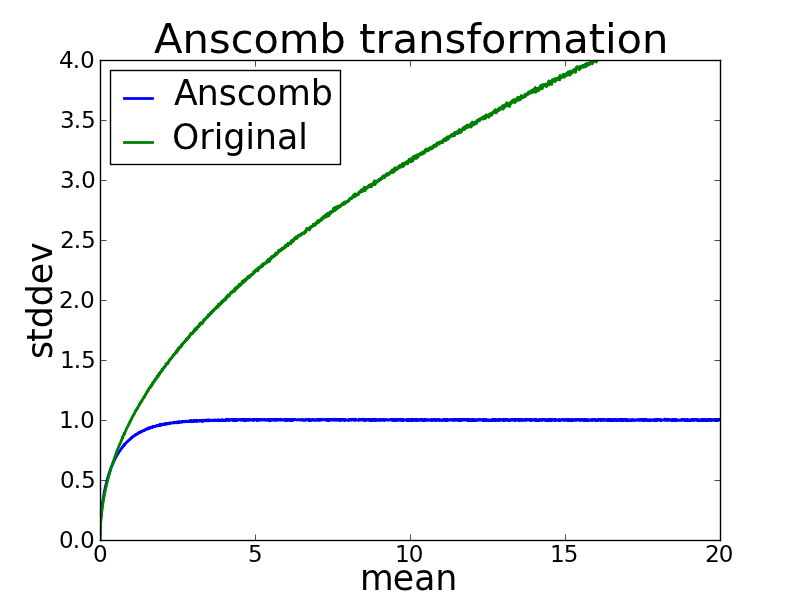
\includegraphics[width = 0.5\textwidth]{pictures/anscombe.png}
	\caption{Standard deviation over mean intensities of different Poisson
	distributions (green) and their Anscombe transformed distributions (blue)}
	\label{anscombe}	
\end{figure}
 

\section{Estimation of camera gain and offset}\label{estimationCameraGain}
Two different ways of estimating the camera parameters have been investigated. For both approaches it is assumed that the intensities of the background and of the beads are Poisson distributed. This data $I_\text{true}$ is then transformed in the following way:
\begin{equation}
	I_\text{meas} = g \cdot I_\text{true} + o \label{trafoGain}
\end{equation}
This is the inverse transformation of equation \ref{transtopoiss}.
\subsection{Using variance-mean plot} \label{skellam1}
The approach for the parameter estimation using the variances of the pixels is shown using a minimalistic example. It is then used in a generalized form.\newline
Consider two pixels with different Poisson distributions $P_1$ and $P_2$ with mean value and variances of this distributions $\lambda_1$ and $\lambda_2$. If these distributions are transformed as given in equation \ref{trafoGain} their mean and variance in temporal domain change as as follows:
\begin{align}
	\text{var}(I_{\text{meas}1})& = g^2\cdot\text{var}(I_{\text{true}1}) \label{calcvar}\\ 
	\text{var}(I_{\text{meas}2})& = g^2\cdot\text{var}(I_{\text{true}2})\\
	\text{mean}(I_{\text{meas}1})& = g\cdot \text{mean}(I_{\text{true}1}) + o\\
	\text{mean}(I_{\text{meas}2})& = g\cdot \text{mean}(I_{\text{true}2}) + o
\end{align}
This allows to determine the gain and offset using only two pixels.
The values for $\text{var}(I_{\text{meas}1}), \text{var}(I_{\text{meas}2})$, $\text{mean}(I_{\text{true}1})$ and $\text{mean}(I_{\text{true}2})$ can be calculated from the data and can be used to calculate the gain as follows:
\begin{align}
	\frac{\text{var}(I_{\text{meas}1})-\text{var}(I_{\text{meas}2})}{\text{mean}({I_\text{meas}1})-\text{mean}(I_{\text{meas}2})}&= \frac{g^2\cdot \lambda_1  - g^2\cdot \lambda_2 }{g\cdot \lambda_1 + o - (g\cdot \lambda_2+o)}\\
	& = \frac{g^2\cdot(\lambda_1-\lambda_2)}{g\cdot (\lambda_1-\lambda_2)}\\
	& = g
\end{align}
The offset $o$ can be calculated in the same way.
\begin{align}
	\text{mean}(I_{\text{meas}1}) - \frac{\text{var}(I_{\text{meas}1})}{g} &= g\cdot \lambda_1 + o - \frac{g^2\cdot\lambda_1}{g}\\
	&= o
\end{align}
The estimation gets more stable if more than two points are used and if the points are taken from a wide range of intensities. If more than two points are used a straight line must be fitted through them. This lines slope gives the gain factor and the intersection on the $x$-axis the offset. The variance of the pixels intensities are calculated directly, instead of using the Skellam approach. This is motivated in section \ref{skellambettervariance}.
\subsection{Using skewness of Poisson distribution}
A second approach is to use the skewness of the Poisson distribution to estimate the mean value.\newline
For every pixel there are multiple intensities in temporal dimension. One can
calculate mean and variance of the measured intensities for each pixel $I_\text{meas}(i,j)$ and
gets
\begin{align}
	\text{mean}(I_\text{meas}(i,j))& = g\cdot \text{mean}(I_\text{true}(i,j)) + o \label{meanvarPoiss1}\\
	\text{var}(I_\text{meas}(i,j))& = g^2\cdot\text{var}(I_\text{true}(i,j)) \label{meanvarPoiss2}
\end{align}
Assuming a Poisson distribution as the true intensity, mean and variance would
be the same. Unfortunately the mean true intensities are unknown and it is
not possible to determine $g$ and $o$ so far. For large mean Intensities $\mu$
the Poisson distribution becomes more and more symmetric and therefore similar to a Gaussian distribution
with the same mean and variance as the Poisson distribution. However, for small means, the Poisson distribution is not
symmetric. The skewness $s_p$ of a Poisson distribution is the inverse of the
square root of the mean $(\mu)^{-.5}$. It can also be directly
calculated from data
\begin{equation}
	s_p = \frac{1}{n}\sum_{i = 1}^n \left(\frac{x_i - \bar x}{\sigma}\ right)^3
\end{equation}
The skewness is invariant to shift and multiplication with a constant. This
means that the transformation caused by the camera gain and the offset
does not affect the skewness. This gives a third equation to solve for $g$ and
$o$.\\
This approach is strictly limited to, at least for background pixels, low intensities. Tests have shown that if the mean of the true Poisson distribution is higher than roughly 30, the skewness gives no stable results. This is shown in section \ref{skewnesssucks}. For data sets with high background intensities it is not possible to determine the camera parameters in this way.

\section{Check for correct gain factor} \label{checkGain}
The gain factor may have been determined or entered incorrectly. Assuming there is the true gain factor $g_\text{true}$ and the incorrect gain factor $g_\text{false}$. Let be Poiss$(\mu)$ the true Poisson distribution of one background pixel and $o$ the offset. The pixels raw intensities are therefore $g_\text{true} \cdot \text{Poiss($\mu$)} + o$. The following shows the effects of the incorrectly chosen gain factor on the transformed images:
\begin{align}
	\frac{(g_\text{true} \cdot \text{Poiss($\mu$)} + o)-o}{g_\text{false}} &= \underbrace{\frac{g_\text{true}}{g_\text{false}}}_{r}\text{Poiss($\mu$)}&\text{Transformation \ref{trafoPoiss}}\\
	2\sqrt{r\text{Poiss($\mu$)}+\frac{3}{8}}&\approx \text{Gauss}(2\sqrt{r\mu},r)&\text{Transformation \ref{trafoAnscombe}}
\end{align}
The variance of the Gaussian can be determined. Since the incorrect estimate of the gain factor and the Gaussians variance $r$ are known, the correct gain factor can be determined by multiplication of the incorrect one with $r$.

\section{Filters}
\subsection*{Gaussian filter}
The Gaussian filter uses a Gaussian for the convolution with the image that shall be filtered. The convolution of an image with a Gaussian filter alters the intensities of the pixels by adding some fraction, depending on the parameters of the filter, of the intensities of the surrounding pixels. The Gaussian filter can be used for noise suppression.
\subsection*{Wiener filter}
The Wiener filter is also known as Wiener-Kolmogoroff filter. One application of the Wiener filter is noise suppression. It is designed to minimize the mean square error of the filtered image compared to the original image without noise. 